\documentclass[a4paper,12pt]{article}
\usepackage{amsmath,amssymb,amsfonts,amsthm}
\usepackage{tikz}
\usepackage [utf8x] {inputenc}
\usepackage [T2A] {fontenc} 
\usepackage[russian]{babel}
\usepackage{cmap} 
\usepackage{gensymb}
\usepackage{float}

% Так ссылки в PDF будут активны
\usepackage[unicode]{hyperref}

% вы сможете вставлять картинки командой \includegraphics[width=0.7\textwidth]{ИМЯ ФАЙЛА}
% получается подключать, как минимум, файлы .pdf, .jpg, .png.
\usepackage{graphicx}
% Если вы хотите явно указать поля:
\usepackage[margin=1in]{geometry}
% Или если вы хотите задать поля менее явно (чем больше DIV, тем больше места под текст):
% \usepackage[DIV=10]{typearea}

\usepackage{fancyhdr}

\newcommand{\bbR}{\mathbb R}%теперь вместо длинной команды \mathbb R (множество вещественных чисел) можно писать короткую запись \bbR. Вместо \bbR вы можете вписать любую строчку букв, которая начинается с '\'.
\newcommand{\eps}{\varepsilon}
\newcommand{\bbN}{\mathbb N}
\newcommand{\dif}{\mathrm{d}}

\newtheorem{Def}{Определение}


\pagestyle{fancy}
\makeatletter % сделать "@" "буквой", а не "спецсимволом" - можно использовать "служебные" команды, содержащие @ в названии
\fancyhead[L]{\footnotesize Термодинамика и молекулярная физика}%Это будет написано вверху страницы слева
\fancyhead[R]{\footnotesize ФМХФ МФТИ}
\fancyfoot[L]{\footnotesize \@author}%имя автора будет написано внизу страницы слева
\fancyfoot[R]{\thepage}%номер страницы —- внизу справа
\fancyfoot[C]{}%по центру внизу страницы пусто

\renewcommand{\maketitle}{%
	\noindent{\bfseries\scshape\large\@title\ \mdseries\upshape}\par
	\noindent {\large\itshape\@author}
	\vskip 2ex}
\makeatother
\def\dd#1#2{\frac{\partial#1}{\partial#2}}


\title{2.1.6 \\ Эффект Джоуля-Томсона} 
\author{Егор Берсенев} 
\date{22 марта 2016 г.}

\begin{document}
	\maketitle
	\section{Цель работы:}
	\begin{enumerate}
		\item Определение изменения температуры углекислого газа при протекании через малопроницаемую перегородку при разных начальных значениях давления и температуры.
		\item Вычисление по результатам опытов коэффициентов Ван-дер-Ваальса <<a>> и <<b>>.
	\end{enumerate}
	\section{Оборудование}
	Термостат, трубка с пористой перегородкой, труба Дьюара, дифференциальная термопара, микровольтметр, балластный баллон, манометр.
	\section{Теоретическая часть}
	\begin{Def}
		Эффект Джоуля-Томсона --- изменение температуры газа, медленно протекающего из области высокого в область низкого давления в условиях хорошей тепловой изоляции.
	\end{Def}
	Исследуем изменение температуры углекислого газа при его медленном течении через пористую перегородку. Газ из области повышенного давления проходит в область с атмосферным давлением. Величина эффекта Джоуля-Томсона определяется по разности температур газа до и после перегородки.
	Рассмотрим два сечения трубки: до и после перегородки. Пусть через перегородку прошел, для определенности, 1 моль газа, $\mu$ --- его молярная масса. Молярные объемы газа, давления и внутренние энергии в сечениях I и II обозначим как $V_1, P_1, U_1, V_2, P_2, U_2$. Для того, чтобы ввести в трубку объем $V_1$ нужно совершить работу $A_1 = P_1V_1$. Проходя через сечение газ сам совершает работу $A_2 = P_2V_2$.
	\begin{equation}
		A_1-A_2 = \left(U_2+\frac{\mu v_2^2}{2}\right)-\left(U_1+\frac{\mu v_1^2}{2}\right)
	\end{equation}
	Перегруппируем члены.
	\begin{equation}
		H_1-H_2 = \frac{1}{2}\mu\left(v_2^2-v_1^2\right)
	\end{equation}
	Используме выражение для коэффициента Джоуля-Томсона.
	\begin{equation}
		\mu_{\text{Д-Т}} = \frac{\Delta T}{\Delta P} \simeq \cfrac{\cfrac{2a}{RT}-b}{C_p}
	\end{equation}
	Используя связь между $a, b$ и критической температурой найдем:
	\begin{equation}
		T_{\text{инв}}=\frac{27}{4}T_{\text{кр}}
	\end{equation}
	Рассмотрим экспериментальную установку.
	
	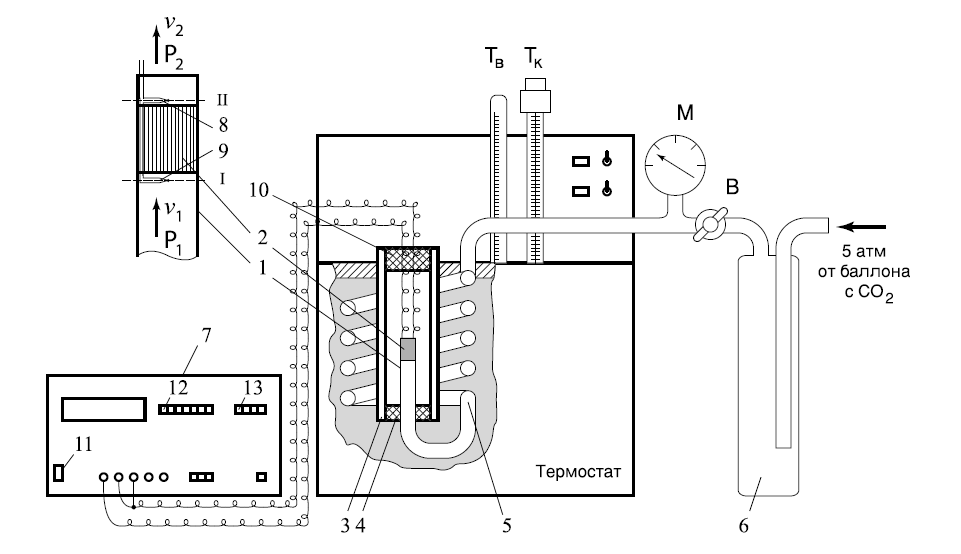
\includegraphics[width = 0.6\linewidth]{instrument}
	
	\begin{enumerate}
		\item Трубка, по которой протекает газ
		\item Пористая перегородка
		\item Труба Дьюара
		\item Кольцо, уплотняющее трубу Дьюара
		\item Змеевик
		\item Балластный баллон
		\item Вольтметр
	\end{enumerate}
	
	\section{Ход работы}
	Включим термостат и вольтметр, снимем значение поправочного напряжения $\eps_0 = 6\,\text{мкВ}$.
	Проведем измерения напряжения на термопаре и  разности давлений:\newline
	

\begin{table}[H]
	\caption{T = 295 K }
	\centering
	\begin{tabular}{  l |  l  l  l  l  l }
		$\Delta P$, атм & 4.1 & 3.7 & 3.3 & 2.9 & 2.5 \\ \hline
		$U-U_0$, мкВ    & 150 & 134 & 116 & 98  & 80 \\ \hline
		$\Delta T$, K   & 3.7 & 3.3 & 2.9 & 2.4 & 2 \\ \hline
	\end{tabular}
\end{table}
\begin{table}[H]
	\caption{T = 313 K }
	\centering
	\begin{tabular}{  l |  l  l  l  l  l }
		$\Delta P$, атм & 4.1 & 3.7 & 3.3 & 2.9 & 2.5 \\ \hline
		$U-U_0$, мкВ    & 124 & 106 & 88 & 74  & 58 \\ \hline
		$\Delta T$, K   & 3   & 2.5 & 2.1 & 1.8 & 1.4 \\ \hline
	\end{tabular}
\end{table}
\begin{table}[H]
	\caption{T = 333 K }
	\centering
	\begin{tabular}{  l |  l  l  l  l  l }
		$\Delta P$, атм & 4.1 & 3.7 & 3.3 & 2.9 & 2.5 \\ \hline
		$U-U_0$, мкВ    & 90 & 74 & 62 & 47  & 36 \\ \hline
		$\Delta T$, K   & 2.1& 1.7 & 1.4 & 1.1 & 0.8 \\ \hline
	\end{tabular}
\end{table}

	\begin{figure}[H]
	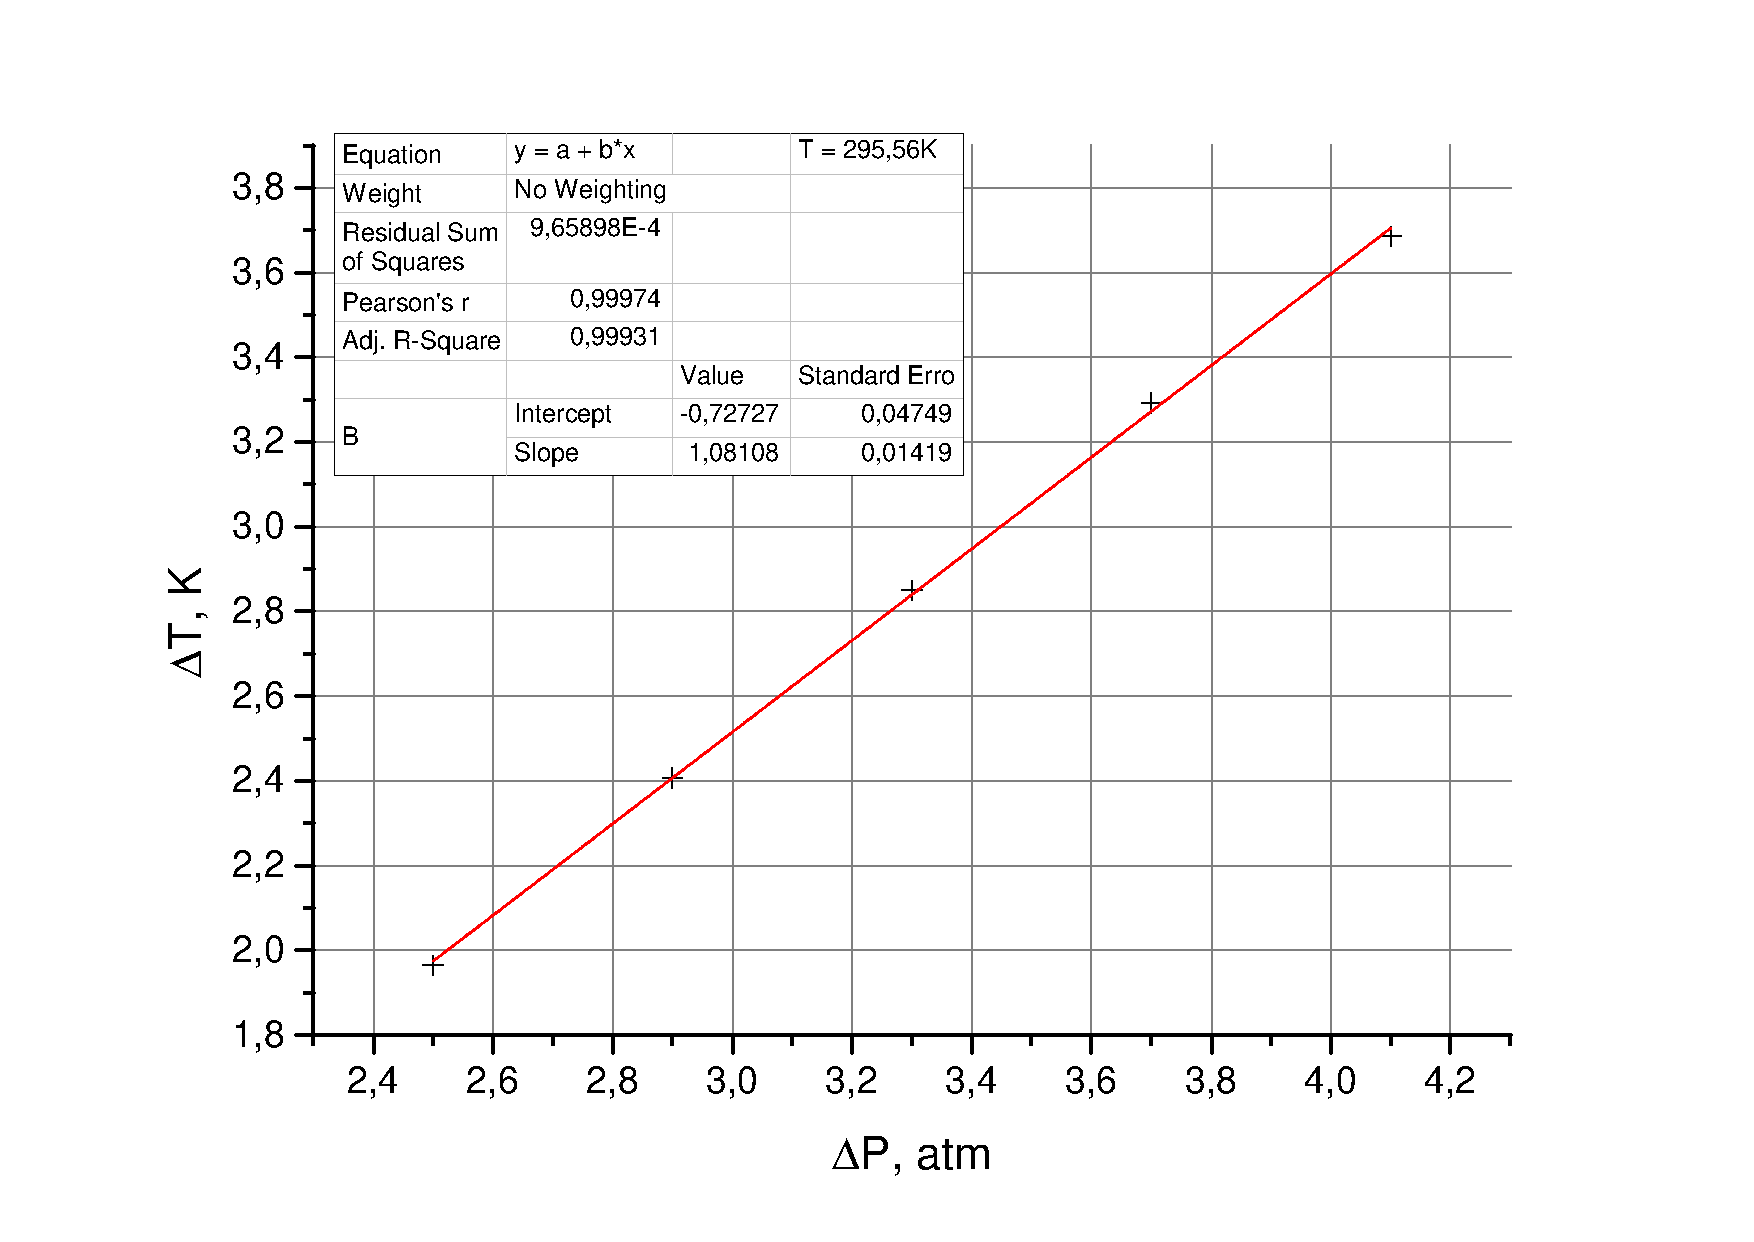
\includegraphics[width = 0.6\linewidth]{295K}
		\caption{T = 295 K}
	\end{figure}
	
	\begin{figure}[H]
	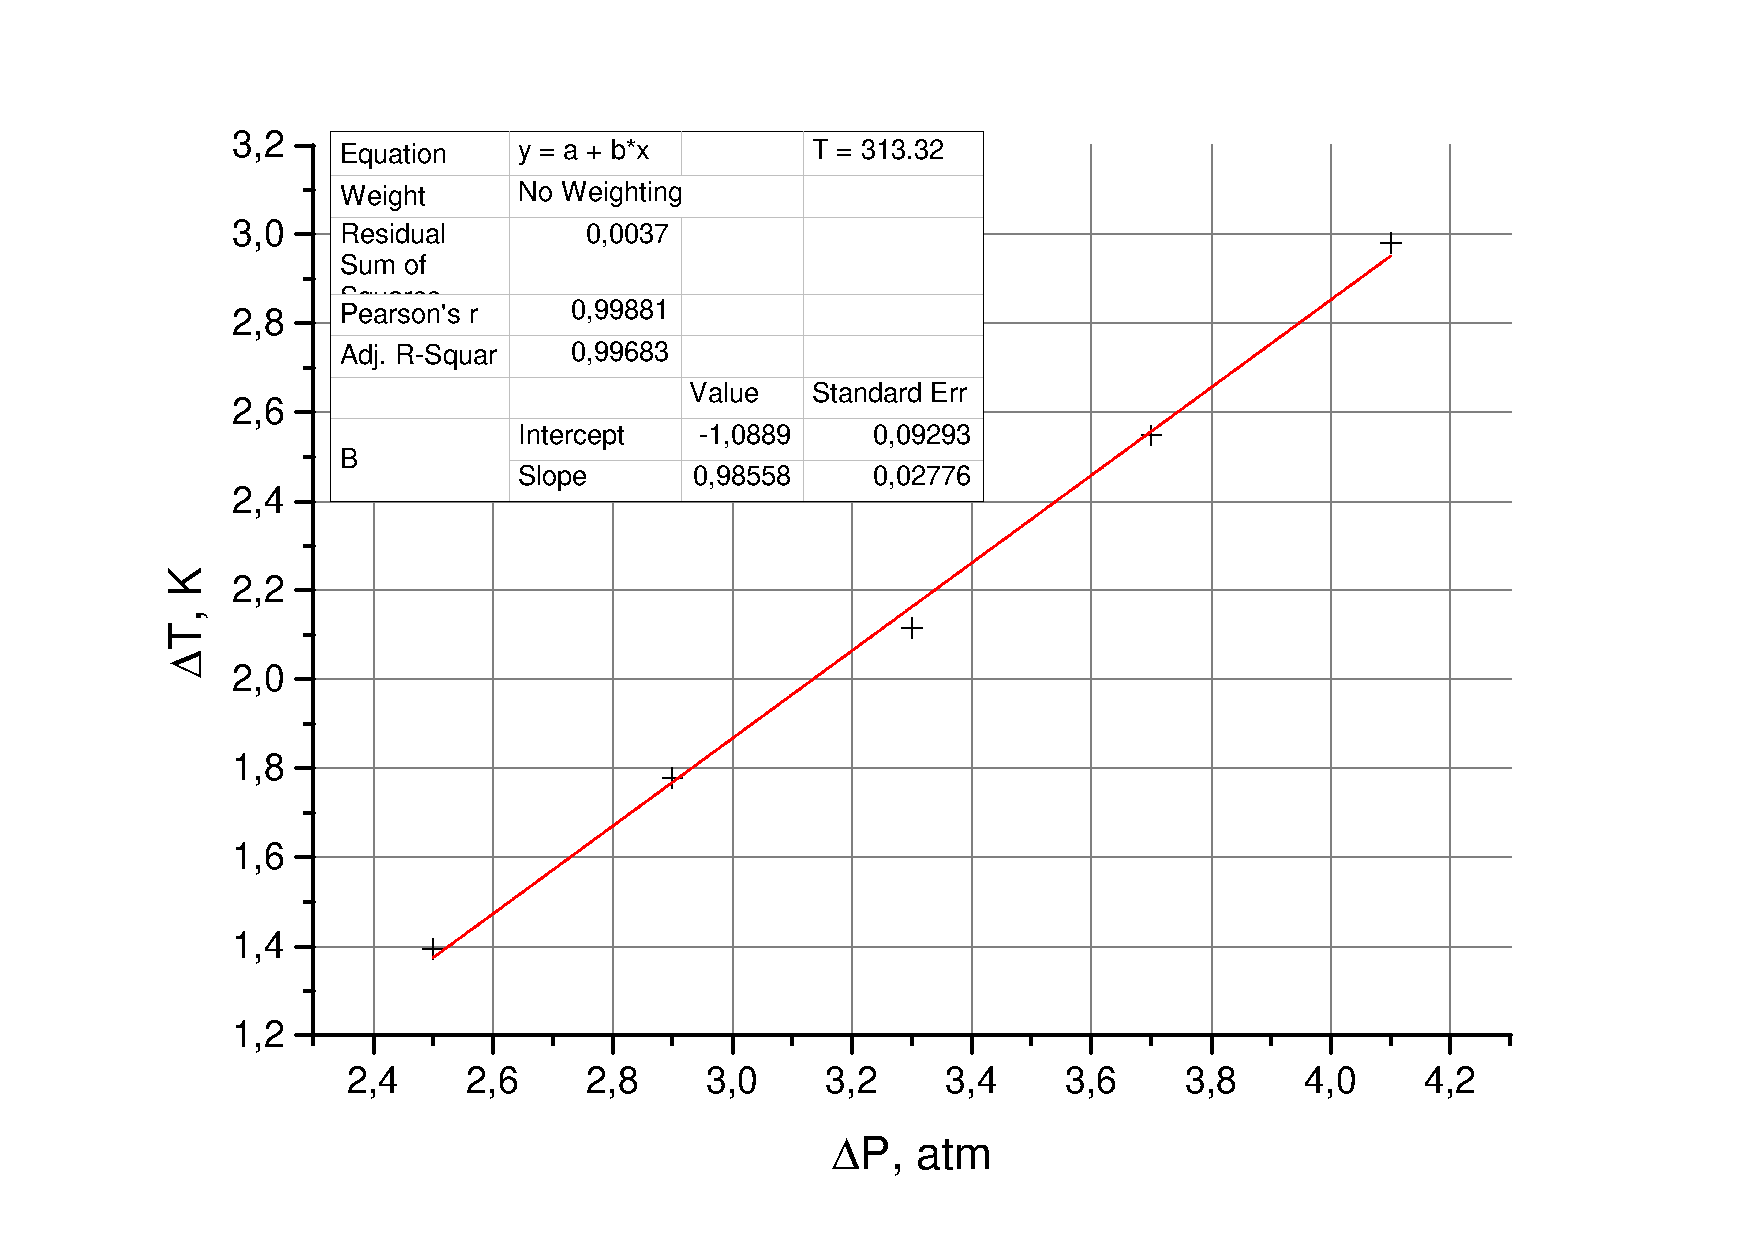
\includegraphics[width = 0.6\linewidth]{313K}
		\caption{T = 313 K}
	\end{figure}
	
	\begin{figure}[H]
	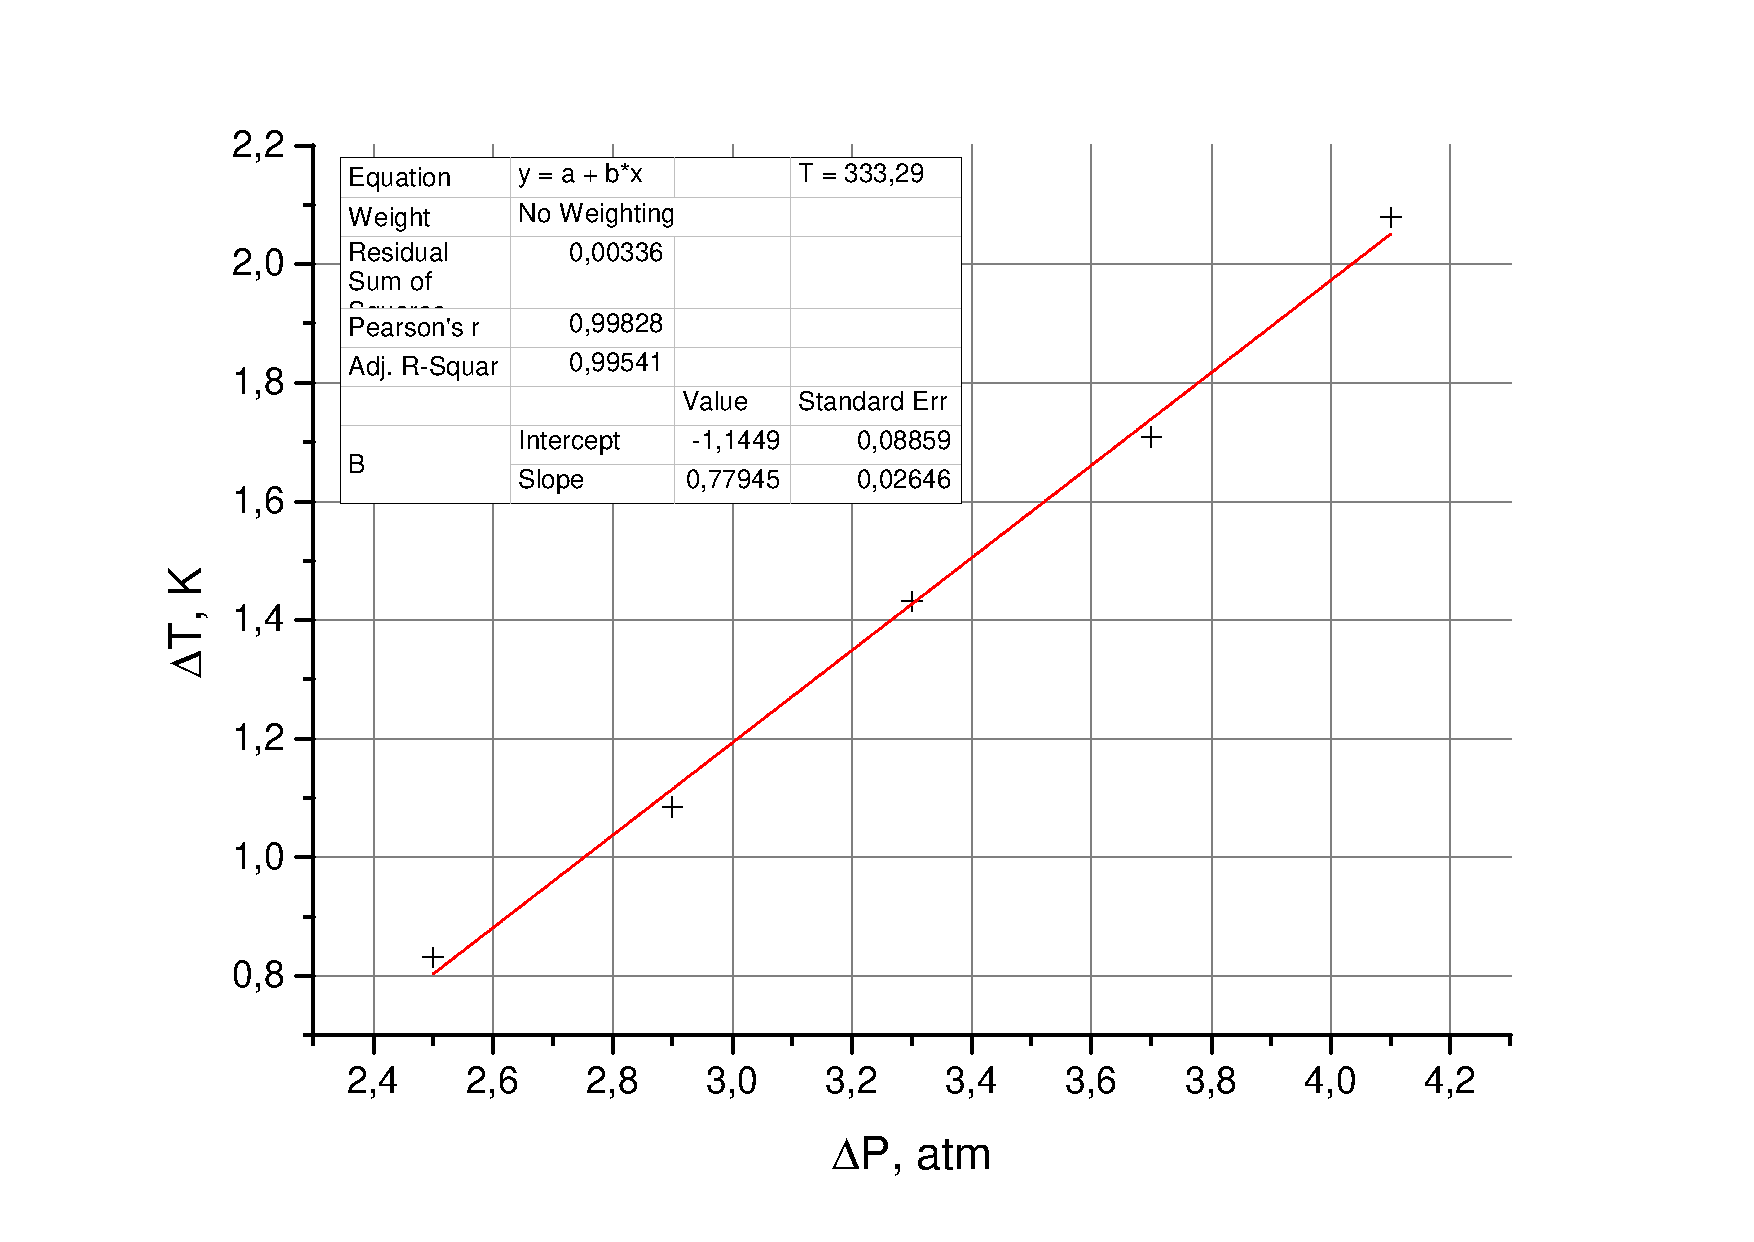
\includegraphics[width = 0.6\linewidth]{333K}
		\caption{T = 333 K}
	\end{figure}
	
	
\begin{table}[H]
	\caption{Коэффициенты Джоуля-Томсона}
	\centering
	\begin{tabular}{  l |  l | l | l }
		 & T = 295 K & T = 313 K & T = 333 K \\ \hline
		$\mu_{\text{Д-Т}}$ & 1.08 & 0.99 & 0.78  \\ \hline
		$\sigma_{\mu_{\text{Д-Т}}} $ & 0.01 & 0.03 & 0.03  \\ \hline
	\end{tabular}
\end{table}

\begin{figure}[H]
	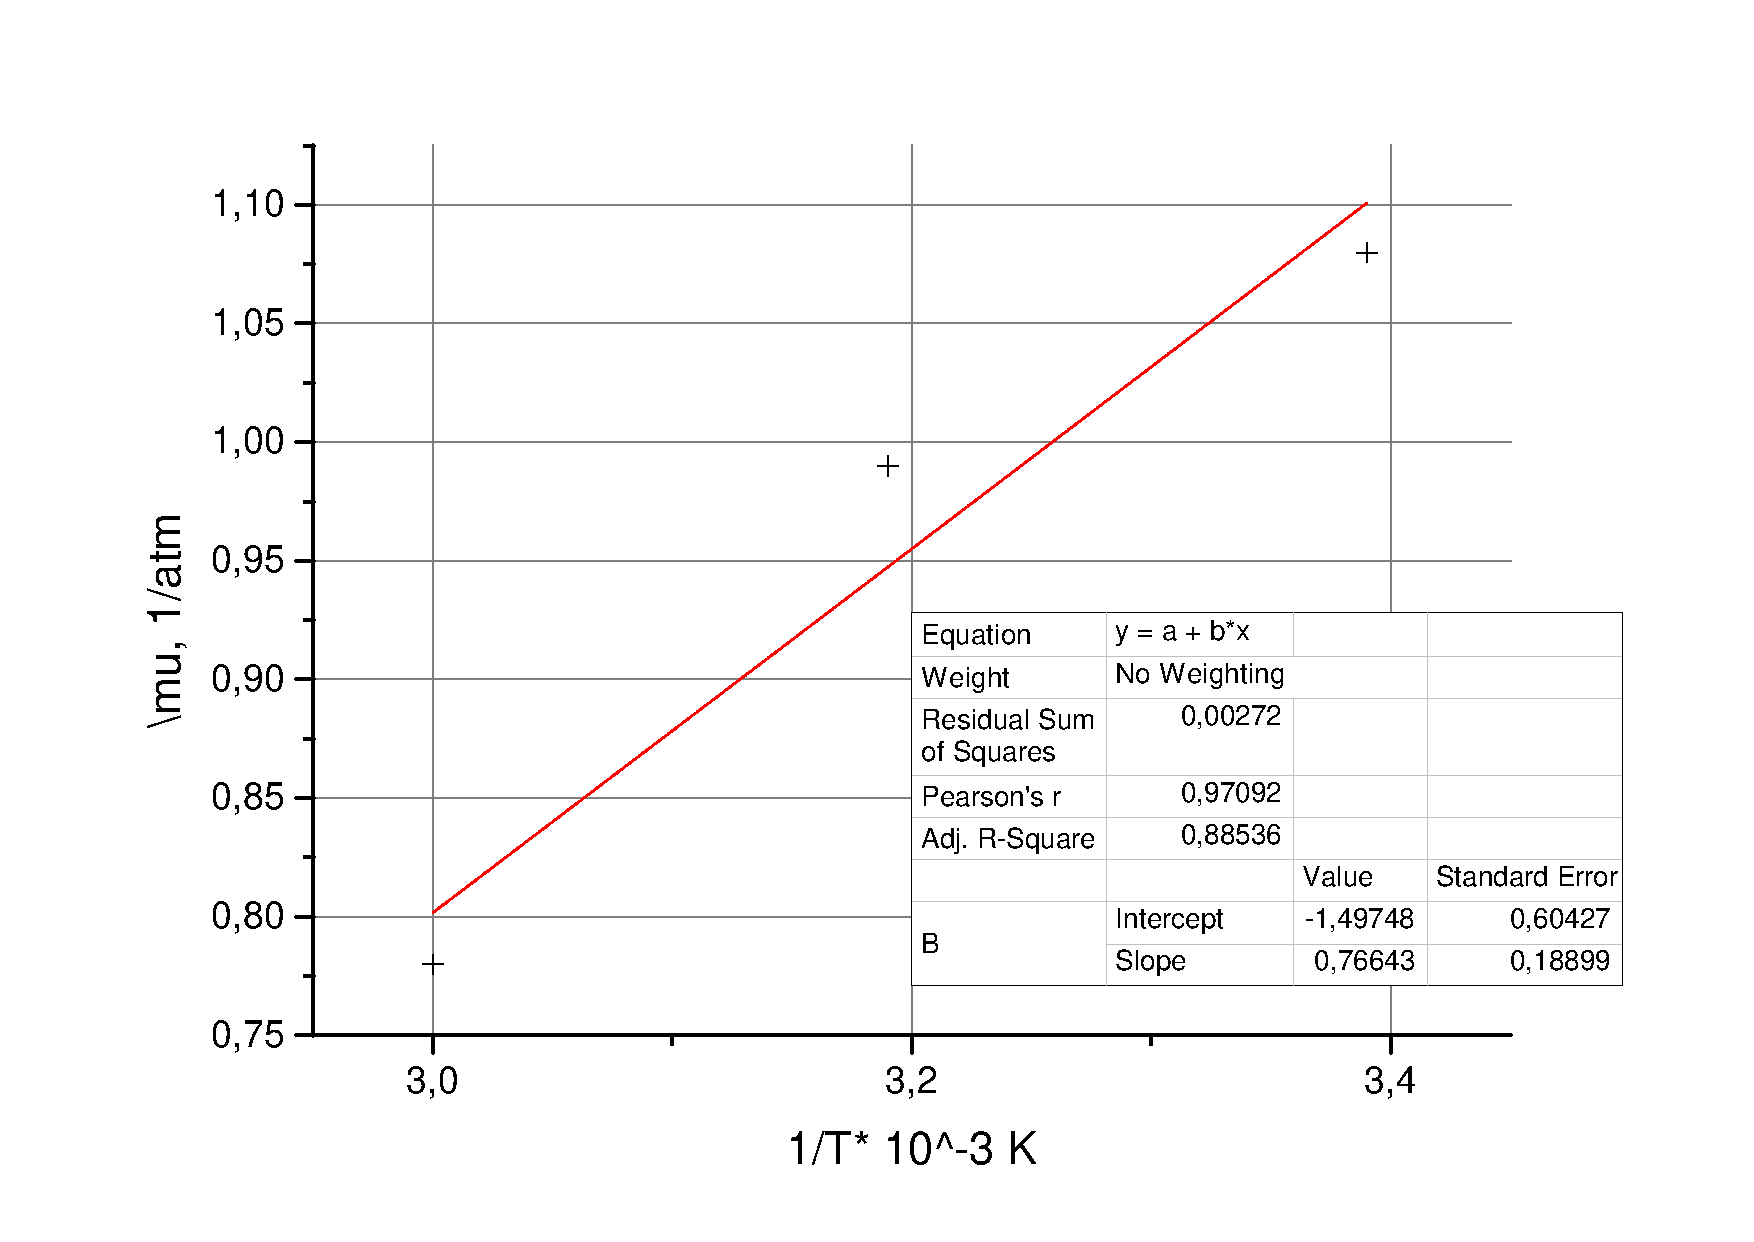
\includegraphics[width = 0.6\linewidth]{mu}
	\caption{Коэффициенты Джоуля-Томсона}
\end{figure}

Коэффициенты Ван-дер-Ваальса $a = \frac{k R C_p}{2} = 1.273 \frac{\text{Н}\cdot\text{м}^4}{\text{моль}^2}$,  $b = -iC_p  =6 \cdot 10^{-4} \frac{\text{м}^3}{\text{моль}}$.


\section{Вывод}
Значения коэффициентов Ван-дер-Ваальса не совпадают с табличными, т.к. в таблице они указаны для критических параметров.
$T_i = \frac{2a}{Rb} = 510 K$, что также очень сильно расходится с табличным. Это могло произойти из-за несовершнества условий эксперимента.
\end{document}



